\chapter{Implementation}\label{ch:problem}
\section{Breaking Down the Problem}
Having examined the state of art developments of \gls{SSGPVS}, what are essentials to successfully make a \gls{SSGPVS} using \gls{RT} simulators and microcontroller is pretty clear. Although theory behind \gls{SSGPVS}  has been studied for quite a long time and there has been existing products on the market already, documentations on development process of a \gls{RT} or \gls{HIL} simulation are still limited. So far the reviews have shed the light on tasks needed to complete the whole project. 

The first task is to develop a \gls{SSGPVS} in the pure software environment which may pave th way for developing a \gls{RT} model for the simulator. The process involved is described in detail in \Vref{sec:build_simulink}. The second issue which is discussed in \Vref{sec:convert_rt} is to revise the model so that it can be load into \gls{RT} simulator and runs in \gls{RT}. 
The third issue is to implement the controller functionalities using a \gls{DSP}. The implementation involves some advanced C language programing which is something I enjoy doing. The details of implementation are presented in \Vref{sec:implement_micro}.
The fourth issue which discussed in \Vref{sec:perform_pil} is to perform \gls{PIL} simulation. This issue is a little bit complicated since it requires me to be well familiar with the real time simulator. And I have not found much resources on this so far. It is a milestone to this project.
\section{Building Model in SIMULINK}\label{sec:build_simulink}
The purpose of a pure software simulation model is to verify the correctness of circuit topology, solar panel model and proper design of LCL filter. Luckily, SIMULINK has a build-in \gls{SSGPVS} model which can be found in \textit{MALTAB 2015B} and later versions\cite{solar_buildin_model}. It provide a good starting point of this project. Since the project focus on performing \gls{RT} simulations, any already known to work model can be used to accelerate the process of building the whole model and save some time avoid doing everything from scratch. 

The model was quite well designed and simulation ran with not error. Minor adjustment may be made before turning it into a \gls{RT} model. The system was design for North America market which result in a 60 Hz operation of grid frequency. Since the grid voltage in Australia is 50 Hz, the grid frequency of original model need to be change to 50 Hz. In order to change the frequency, the minimum time step, \gls{PWM} frequency of the inverter and controller sampling time need to be changed as well. The reason for changing the minimum time step is that fixed time solver for solving ordinary differential equations(ODE) is used for simulation which means grid frequency, controller sampling time or any other components' sampling time need to be integer multiple of minimum time step. \Vref{tab:change_list} is a summary of different configurations between models. 
\begin{center}\label{tab:change_list}
\begin{tabular}{ |c|c|c| } 
 \hline
 Items Changed & Origin Configuration & New Configuration\\ \hline
 Minimum time step &  $1.323e^{-6}$ s & $6.25e^{-7}$ s \\ \hline
 Carrier frequency & 3780 Hz & 8000 Hz\\ \hline
 Controller sampling & $2.6455e^{-5}$ s& $1.25e^{-5}$ s\\ \hline
\end{tabular}
\end{center}

Noticing that the switching frequency is set to 8 kHz because higher switching frequency may lead to less bulky inductors in real life which is less expensive. Instead of setting switching frequency to nearer 4 kHz, double of the frequency is chosen. In order to ensure the accuracy of simulation and avoid limited resolution on duty cycle, $6.25e^{-7}$ s of minimum time step has been chosen to ensure minimum stepping of duty cycle is 0.5\%. The duty cycle resolution could affect \gls{SSGPVC} creating high output current THD and undesired phase shift since duty cycle can only vary in discrete steps.

Changed made in \gls{PWM} frequency lead to smaller minimum time step, thus, more time needed to generate one second simulation results. The time it takes to run the simulation depends on configurations of the host PC and it is common to run simulation for around five minutes to generate one second of results. 

The controller design in the model is different from what has been mentioned previously. Bearing in mind that the purpose of using this model is to obtain a working plant for performing \gls{RT} simulation in the next stage, as a result, the design of the controller is not thoroughly studied. 

\section{Convert to Real-time}\label{sec:convert_rt}
After getting a working model running in SIMULINK, the model should be convert to \textit{RTLAB} compatible model. Currently, \textit{RTLAB} only support \textit{MATLAB 2014B}, the first thing to do is to make sure the model can still work under \textit{2014B}. Unfortunately, the model makes use of a generic solar \gls{PV} model which is only rendered in \textit{2015B}. In order to continue doing simulation, the \gls{PV} model need to be replaced with a replica.

\subsection{Custom Solar Cell}
Since access to source code to \textit{MALTAB}'s PV panel model is not possible, creating a replica of the \textit{MALTAB}'s model is important so that it would be possible to verify the custom solar cell model is acutally correctly implemented. Based on what has been stated in \Vref{sec:solar_cell}, the custom model was initially built up in a script in \textit{MALTAB}. Since scripts or functions written in \textit{MATLAB} is also compatible to run using SIMULINK, it should not be difficult to integrate the script into existing \gls{SSGPVS} model. 

The initial idea was to implement a generic \gls{PV} cell which only relies on some key parameters that represent the external characteristic of the cell. The parameters include open circuit voltage, short circuit current and temperature coefficients of voltage/current. As for the internal serial and parallel connected resistors, they may be obtained via proper calculation. In this way, the model can be easily extended to simulate any cell or panel of interest. However, how to archive this goal is not clear at the time when the model was implemented since the resistors' value are usually acquired via measurements made by the manufacturers of of the cell/panel. Not many article which is available shed light on how to accurately estimate those parameters from external characteristic of cell/panel, which makes it difficult to fulfill this goal. As a workaround, the model was implemented under the condition that the two parameters are provided by the manufacturer, otherwise there is no way to implement the model. 

The first version of the cell model was implemented as a completely standalone model (black box) which does not reply on any \simulink~models. The first trial was based on \cite{RN26} since the model it proposed is simple and easy to understand. However, the model in the article is a simplified one which shunt resister is not considered. Also, Newton's method was used to derive serial resistor value of the cell, of which is based on iteration. Newton's method may fail to converging to local minimum point when variables are trapped in saddle points. 
\cite{RN24} has more details on models which have different levels of simplification and equations are well presented. This makes it easier to understand and implement the model. Model presented in \cite{RN24} were built-in native \simulink~, however, using 'drag and drop' method has limitation on the maximum efficiency that one can archive. That's the reason that custom model implemented in this project is written as a script and the running results are presented in the later chapter.

It turned out that the idea to make the model as a black box is not a good idea because this approach makes it hard to interface with the rest of the system in \simulink~. Interestingly, \simulink's way of modeling a circuit system is different from doing numerical calculations. It is not possible to directly interface circuit models with numerical calculation blocks. Custom components need to be implemented using controlled voltage or current source. Considering the design rules imposed by \simulink, there is no choice but to implement custom model partially based on \simulink~native blocks (mainly controlled sources) to reuse most of work has been finished before. 
\begin{figure}[h]
     \centering
     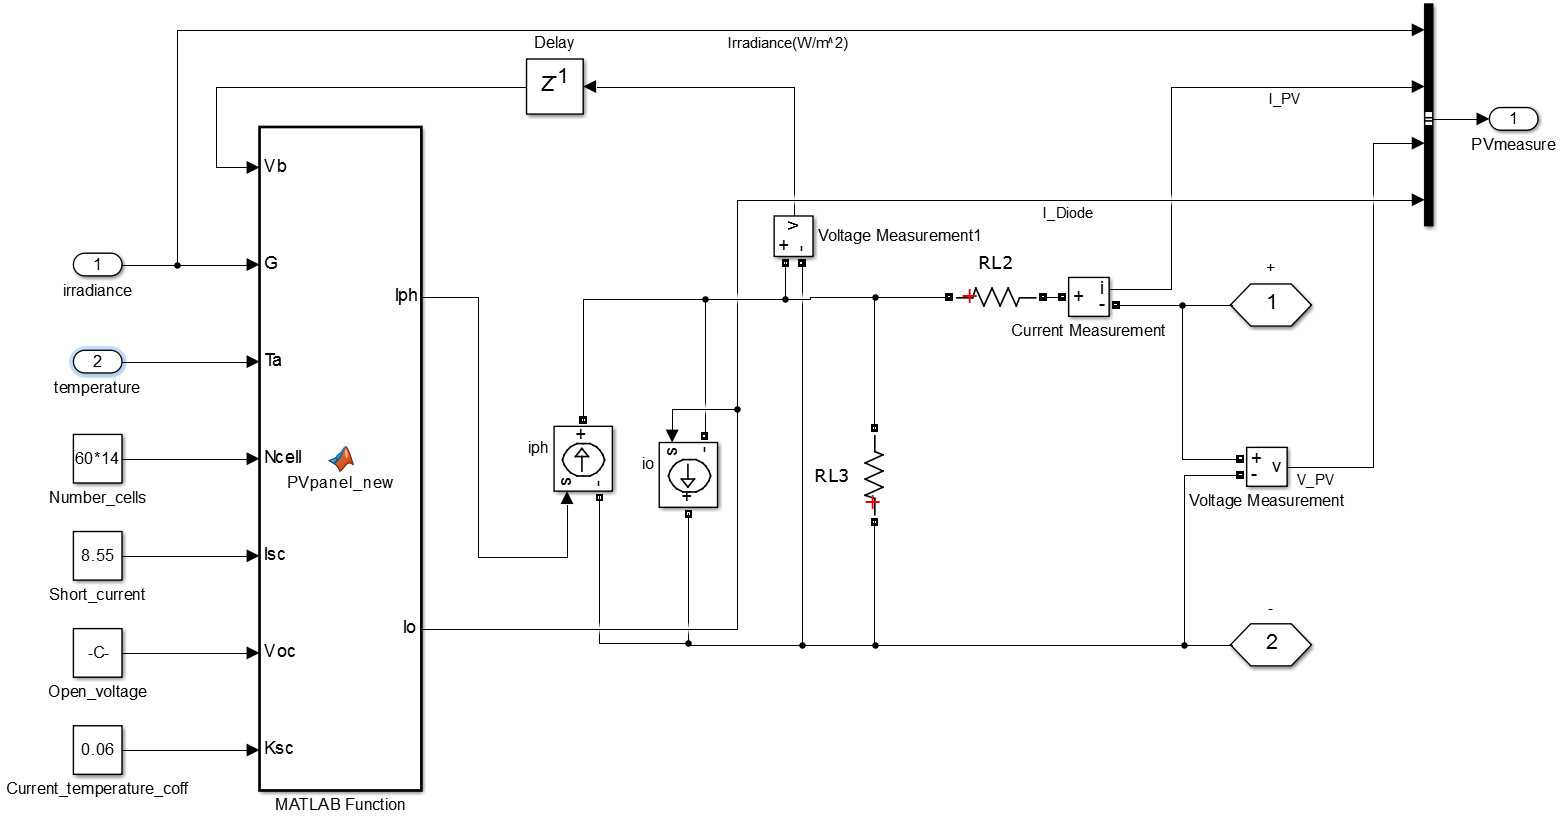
\includegraphics[width = 1\textwidth]{figures/custome_pv}
     \caption{Custom solar cell model}
     \label{fig:cell_model}
\end{figure}

\Vref{fig:cell_model} illustrates the final version of custom solar cell model and it is a replica of model that used before. Algebraic loop which is often the reason why simulation cannot run is a critical issue encountered during the process of making the model. Examining Equation \ref{equ:solar cell} carefully, it is not hard to find that output current of solar cell depends on terminal voltage of the cell. The terminal voltage, in turn, depends on output current flow through external load. This means that in order to calculate either of them, at least one parameter has already been known,  which forms a classic algebraic loop. For the sake of running simulation, algebraic loop need to be broken by introducing delays into the system. The presence of a delay module in \Vref{fig:cell_model} is to break algebraic loop and setting up initial condition properly. Sometimes, extra delay may lead to unstable operation of the system, however, it is not a problem with custom model fortunately.

\subsection{RTLAB}
As menstioned before, \gls{RT} model should be able to run using RTLAB because RTLAB is the only software that is capable of communicate with Opal-RT's simulators. The workflow to work with RTLAB is listed below. 
\begin{enumerate}
\item \textbf{Create a new project} \\
New project should be created with human readable project name. This would create a new folder to hold all the project related files including \gls{RT} models and configurations and completions. 
\item \textbf{Import exisitng model} \\
Two options are available during this stage, one is template model provided by the Opal-RT, the other one is directly import the known to work model created previously. For a brand new pure software model, it is recommended  to import the templates, then copy the pure software model into the template. In this way, users do not need to configure all the settings from scratch, however, caution need to be taken because some configurations may not be suitable for any models. 
\item \textbf{Moidify model} \\
Once imported, users should be able to edit the model via \rtlab~ launched \matlab~ window. There are some requirements imposed by \rtlab~ and users need to make sure the model should be able to compile and run offline (without loading onto simulator). Since \rtlab~ is not smart enough at the moment, it needs users' help to separating model into different functional blocks so that each functional blocks can use one processing core in the simulator to maximize performance by running simulation in parallel. Different cores may communicate with each other synchronously or asynchronously depends on users' preference. 
\item \textbf{Build \gls{RT} model} \\
The reason for this step is that simulator cannot run \matlab~ model directly (and should not). In fact, \simulink~as a high level development environment, has relatively low efficiency running time critical simulation. However, with the help of \matlab~ coder, \simulink~models can be compile into C/C++ which is a low level language that can be run of high efficiency. Generated files are stored in the project folder and once all completions are ready users may continue. 
\item \textbf{Load model and perform \gls{RT} simulation} \\
In this stage, all completions are transferred from host PC to simulator and \rtlab~ would put simulator into ready state. Once users click on button to start simulation, simulator would start running and user may use auto-generated console window to interact directly with the simulator. Users may choose to pause or stop simulation at anytime via \rtlab.
\end{enumerate}
\subsection{\ehs}
\ehs is a generic and reconfigurable FPGA-based electrical solver which provides a convenient user interface enabling users to bring into \gls{RT}models created in the simulation tool of different mainstream simulation environment including \simulink, PSIM, PLECS Blockset, and Multisim. \ehs operate at a much finer time resolution, so communication between \ehs and \gls{CPU} cores is archived by sampling. At the beginning of each calculation, \ehs solver samples the values in \gls{CPU} and perform calculations based on the sampled values. 

In \simulink, \ehs solver is represented as a block diagram and it contains many parameters that users may like to change. Here are some differences between building a regular \rtlab~ model and \ehs model.
\begin{enumerate}
\item \textbf{Separate model into two files} \\
\rtlab~ allows users to put models from \textit{SimScape Power System \simulink~toolbox} together with normal numerical calculation block under the same subsystem. The idea behind separation of simulation file is still the same. Because \rtlab~ and \ehs are not that smart, they need manual process of separation. Briefly, \ehs is able to handle majority of circuit models in \textit{SimScape Power System toolbox}. Instead of separate those models into subsystem under the same file, they need to be separated into two different files.  The rest of the system, apart from those power system models, become master of model and interface with power system models with \ehs block diagram. 
\item \textbf{Changing naming of used power system models} \\
\ehs makes use of pre-generated \gls{FPGA} firmware that have special requirements on naming of each modules used in simulation model. By following the naming convention, model translator is able to map each modules onto different sections of digital circuit that take advantage of parallel computation power rendered by \gls{FPGA}. 
\end{enumerate}
\section{Implementation In Microcontroller}\label{sec:implement_micro}

\Vref{fig:software_flow} illustrates software flow implemented in TMS320F28027(F28027). Since objective of this project is to implement a simple \gls{SSGPVS} and perform \gls{HIL} simulation to prove the concept of fast prototyping and development without real hardware, only the necessary elements are implemented in the \tms. It is quite convenient to extend the program to archive much more functionalities depends on requirements. For example, communication via  Universal Asynchronous Receiver/Transmitter(UART), power line communication, and temperature sensing can be added into background tasks section to make it more realistic and closer to actual product. 
\begin{figure}[h]
     \centering
     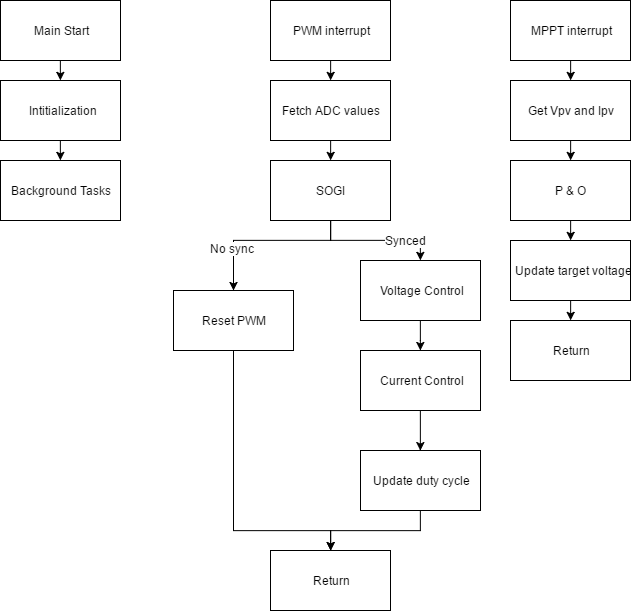
\includegraphics[width = 0.9\textwidth]{figures/software_flow}
     \caption{Software flowchat}
     \label{fig:software_flow}
\end{figure}
\subsection{IQ math and Computation Budget}
Due to the fact that our microcontroller is a fixed point microcontroller, there is no floating point processing in \tms. We cannot execute any floating point arithmetic using \tms, however, it is still possible to use float point numbers when writing codes. Compiler has the ability to handle the situation to perform float point calculations using software implemented floating point library. The performance is largely sacrificed because what the software floating point library does is to calculate floating numbers using \fp~ using iterative numerical methods. Depends on implementation of software library, multiplications on microcontroller might take so long that in hard \gls{RT} applications program can fail to meet computational deadline. Especially for digital control of power electronic applications, modern designs call for higher and higher \gls{PWM} frequency in order to minimize size of passive components, thus, increased bandwidth requirements for controllers. 

Fortunately, \tms~has 32x32 and 16x16 Multiply-accumulate(MAC) units inside that offer possibilities to do multiplication using less than 10 clock cycles, which make it promising for \gls{SSGPVS} applications with a reasonable \gls{PWM} frequency. In order to make use of MAC, software developers need to code in assembly because compiler might not be able to directly translate \fp~ multiplications into assembly efficiently. to squeeze every possible improvement on performance. Usually development in assembly is extremely time consuming and violate origin purpose of fast prototyping. Texas Instruments provides IQ math library as a solution to avoid dilemmas like this. Using the library can ensure that all multiplications can make the most of MAC available. The advantage of using this library is that it is straightforward and relatively simple. the disadvantage is that level of accuracy is not guaranteed. The following table has some key math operations and their benchmarks\cite{iqmath_lib} which are used intensively in the program. 
\begin{center}\label{tab:iqbench}
\begin{tabular}{ |c|c|c| } 
 \hline
Math operations & Execution cycles & Program memory (words)\\ \hline
$\sin$ &  46 & 49 \\ \hline
$\cos$ &  44 & 47 \\ \hline
magnitude &  86 &  96 \\ \hline
square root &  63 & 66 \\ \hline
multiplication &  7 & N/A \\ \hline
division & 63 & 71 \\ \hline
\end{tabular}
\end{center}
It is a good practice to avoid as much division as possible because cost of doing division is ten times higher than doing multiplication according to Table \ref{tab:iqbench}. Usually, instead of doing division directly, same operation can be archived by doing reciprocal of divisor. 

How IQ math work is quite common in Digital Signal Processing(DSP) applications. Basic idea is that processors treat all quantities as integers. Developers are free to choose any scaling factors to enlarger fractional part of a number to a integer. In order to simplify calculation, scaling factors are better to be exact power of 2 because multiplication with number of power of 2 can be archived by doing bit shifting. Bit shifting is much cheaper than normal multiplication in terms of computation. The developer must then bear in mind that the integer values are scaled versions of the original input samples, scaling the output back accordingly. To minimize the impact of integer rounding effects, it is desirable to scale the results produced by each processing step so that they utilize as many of the available bits as possible.

Based on the benchmarks, it is possible to allocate computation budget. After reviewing some of reference design of  microinverter products, it is common that inverter loop running in the controller can archive bandwidth of 50 kHz. Although the microcontroller used in the reference design\cite{inverter_ref} has better performance compared with \tms, it would be still interesting to see whether it is possible to complete the jobs using a lower end microcontroller. 

Firstly, the target bandwidth is the same as reference design, ie. 50 kHz. Assume \tms~operate at maximum clock speed which is 60 MHz, timer with 60 MHz clock input is used to generate interrupts at 50 kHz and all computations are complete in interrupt service routine(ISR). Counter value can be calculated using the following equation. 
\begin{align}
    value = \frac{F_{clk}}{F_{loop}}
\end{align}
where ${F_{clk}}$ is the clock frequency that drives the counter, $F_{loop}$ is the control loop frequency. In this case, the value is 1200, which means all tasks in inverter control ISR need to be finished using clock cycles less than this value. Also, other tasks including background and slow loop ISR need clock cycles to execute. After finishing first version of the program, for inverter control ISR alone, there are 24 multiplications, two trigonometric operations, one magnitude operations and one division in total which sum up to execution clock cycle of 409. Other operations or factors need to be considered are summation, conditional operation, function switching overhead, \gls{ADC} sampling time  and on-chip flash synchronization. 

Flash synchronization may lead to excessive overhead because flash is considered to be a slow peripheral that operate at a much more slower speed compared with \gls{CPU} in microcontroller. More than 3 clock cycles of overhead are expected each time the \gls{CPU} perform a visit of flash. On-chip Static random-access memory(SRAM) is an ideal place to store instructions, constants and computation temporals because there is no clock cycles needed to fetch content stored in SRAM. However, integration of large SRAM in silicon is extremely expensive because it is huge in size compared with other parts of circuit, which means there is limited SRAM and it is not possible to put everything in SRAM for a low end microcontroller. Only time critical part of code may be put in SRAM to archive high performance.

Considering all have been stated above, the microcontroller may not has sufficient capabilities meet timing deadline and overruns are highly expected. In order to be safe, halved original frequency looks like a better choice now. \tms~would definitely have abilities to finish all tasks within time.

\subsection{Peripherals Configurations}
There are two important peripherals that are critical to the implementation of the controller, \gls{ADC} and timers. \gls{ADC}
is used to convert analog signals(voltage and current) into digital signal so that \gls{CPU} can use those sample values to perform calculations to control H-bridge. Timers are important because generation of \gls{PWM} as well as ISR rely on proper functioning of timers. 

According to \cite{adc_ref}, the core of the \gls{ADC} contains a single 12-bit converter fed by two sample and hold (SH) circuits. Simultaneously as well as sequentially sampling of the SH is possible. SH are controlled by 16 identically Start-Of-Conversions(SOC) units. Developers only need to configure the SOC units and it would take care of the sampling. SOC can be configured to working with either SHs and there are multiple sources to trigger \gls{ADC} sampling. In this project, since there are four analog channels need to be sampled which mean at least 4 SOCs are needed. During implementation, five SOCs in fact are used because the first value of ADC sampling may be incorrect according to errata\cite{tms_errata} published later. The first SOC is used to control SH to sample analog channel twice to ensure the result is correct. The trigger source of SOCs used is Timer One(T1) which is the same timer to generate \gls{PWM} signal. When triggered at the same time, SOC with smallest identification number (SOC0) has the highest priority to access SH and do conversion. At the end of each conversion, an interrupt of end-of-conversion is generated and \gls{CPU} has to response to the interrupt. 

Timer of \tms~is extremely powerful, since our \gls{PWM} frequency is relatvely low, the high resolution feature is not useful in this case. Each counter modules can be used to generate one pair of complementary \gls{PWM}. Practically, two timers are needed to generate totally four \gls{PWM} signals. However, bipolar modulated \gls{PWM} is used in this case and one \gls{PWM} can be used to control two switches, as a result, only one timer is used which is T1. In order to generate central aligned \gls{PWM} to minimum THD, T1 is configured to work in up-down counting mode. One comparator is used to set and reset the output. If the counting register is equal to comparator register when counter is counting upward, output is set to high. When the counter register's value is equal to value in period register, the counter start to counter downward. When the counter is counting downward, output reset. The following equation is used to calculate duty cycle. 
\begin{align}
    Duty = \frac{Comparator\ value}{Period\ value}
\end{align} 
\begin{figure}[h]
     \centering
     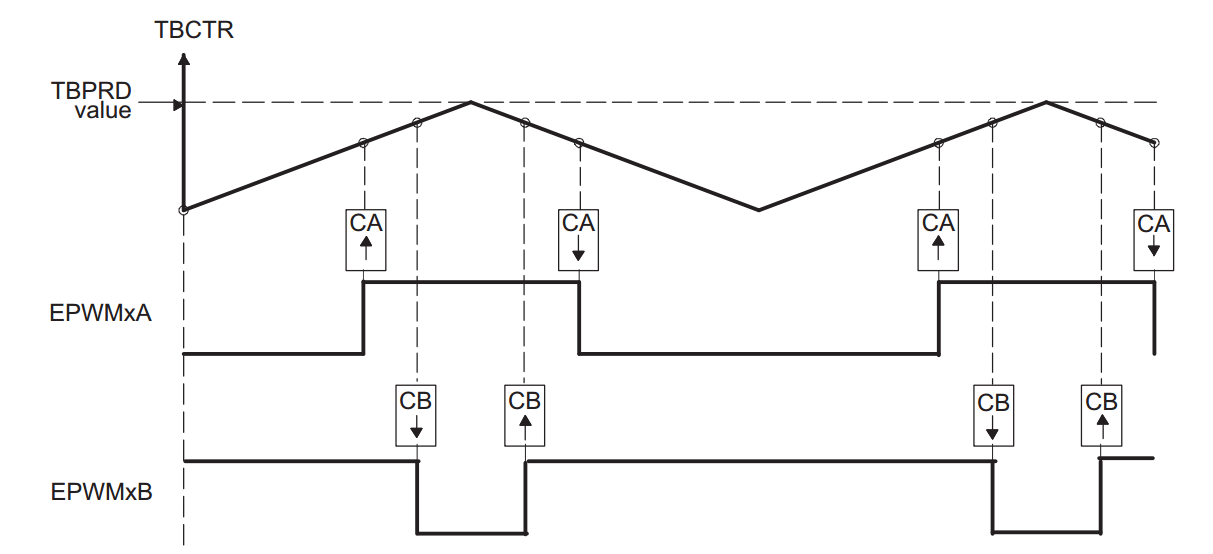
\includegraphics[width = 0.9\textwidth]{figures/timer_wave}
     \caption{Timer waveform}
     \label{fig:timer_wave}
\end{figure}
One advantage offered using up-down counting in this case is that SOC can be triggered when counter value is equal to period value, which means the moment that ADC start sampling is far away from switching moment. During switching transient period, the voltage or current are in transition, which inject undesired noise into system. Sampling during transient period can be extremely noisy and usually people would try this avoid this. Since output impulse is always center aligned with counter peak value. \Vref{fig:timer_wave} illustrate how T1 works in this case. 

In summary, ADC sampling rate of the system is the same as \gls{PWM} frequency and controller bandwidth is also the same in this case since controller functions are called right after sampling finishes. Ideally controller can be set to independent with sampling frequency depending on applications and requirements.
\subsection{Inplement Algorithms}
\gls{SOGI} presented before is in continuous form which is not very helpful since microcontroller works in discrete time. Continuous transfer functions need to be discretize using various method. As mentioned in \cite{RN21}, trapezoidal approximation has a better performance compared with other discretization methods. Discretization operator can be represented using Equation \ref{equ:discrete}.
\begin{align}\label{equ:discrete}
    s = \frac{2(z-1)}{T_s(z+1)}
\end{align}
After doing some math, the discrete time system can be summarize as following. 
\begin{align}
    H_d(z) &= \frac{\frac{x}{x+y+4}+\frac{-x}{x+y+4}z^{-2}}{1 - \frac{2(4-y)}{x+y+4}z^{-1} - \frac{x-y-4}{x+y+4}z^{-2}} = \frac{b_0+b_2z^{-2}}{1-a_1z^{-1}-a_2z^{-2}}\\
    H_q(z) &= \frac{\frac{ky}{x+y+4}+\frac{2ky}{x+y+4}z^{-1}+\frac{ky}{x+y+4}z^{-2}}{1-\frac{2(4-y)}{x+y+4}z^{-1}-\frac{x-y-4}{x+y+4}z^{-2}} = \frac{qb_0+qb_1z^{-1}+qb_2z^{-2}}{1-a_1z^{-1}-a_2z^{-2}}
\end{align} 
where $y= (\omega_nT_s)^2$ and $x=2k\omega_nT_s$. $\omega_n$ is the fundamental frequency, in this case, $\omega_n=2\pi 50=314.2$. $k$ is scaling factor determine the transient response of \gls{PLL}. In the program, $k$ is set to be 0.5. $T_s$ is the sampling frequency or the time interval between two runs of \gls{PLL}.

The current PR controller given in previous chapter is also defined in continuous time domain. Same method, ie trapezoidal approximation, has been used to derive the discrete time system.
\begin{align}
    G_{pr} &= K_p+\frac{K_i\frac{2(z-1)}{T(z+1)}}{\frac{4(z-1)^2}{T^2(z+1)^2}+\omega_n^2}\\
         &= \frac{(K_p+\frac{2K_iT}{(4+T^2\omega^2)})+(\frac{2K_p(T^2\omega^2-4)}{(T^2\omega^2+4)})z^{-1}+(K_p-\frac{2K_iT}{T^2\omega^2+4})}{1+\frac{2T^2\omega^2-4}{T^2\omega^2+4}z^{-1}+z^{-2}}
\end{align}
Transfer function can be implemented reusing the 2 poles 2 zeros system function to make coding easier. 

At the closing stage of this project, harmonic compensators are not added into the current transfer function because adding more transfer functions in parallel makes it hard to debug the system. Turns out that absorbing $K_p$ is not a good practice here because it makes adding harmonic compensation difficult. Developer can take advantage of parallel implementation here to separate origin transfer function into gain $K_p$ part and resonant second order system part $\frac{K_is}{s^2+\omega_n^2}$ to reuse resonant part in code to add harmonic compensation easily. 
\section{Performing \gls{PIL} Simulation}\label{sec:perform_pil}
\subsection{Simulator Output}
The simulator is able to generate two types of output signals, which are analog and digital.

Digital output implemented in the simulator is open-drain which means the output would be able to generate high voltage level without an external power supply. But one advantage offered by this structure is that the output voltage level can be determined by users with proper power supply. 

Analog output is quite straightforward, \rtlab offers a configuration model to let users set channel properties easily. Those properties include upper/lower bound, offsets and scaling, which makes it easy to interface with external circuit. 

\subsection{Simulator Input}
There are two types of input the simulator can accept which are analog and digital. Since microcontroller does not have DAC build-in and there is no use to feed analog signal into simulator. So use of analog input is out of scope for this project. 

The usage of digital input is critical for the success of this project. After examining simulator's device sheets and various reference manuals, there are many different types of digital input to feed digital signal into \gls{CPU} simulation environment. One vital thing developers need to be careful about is the time step of \gls{CPU}. The time step of \gls{CPU} environment imposes maximum sampling frequency of digital input. This is extremely important, particularly for power electronic applications when uses want to feed high frequency \gls{PWM} into the simulator. If the \gls{PWM} frequency is too high, duty cycle resolution may be sacrificed due to sampling effect. The available types of digital input which can be implemented in \gls{CPU} environment are listed below. 
\begin{enumerate}
\item \textbf{Static input} \\
This type of digital inputs is the easiest to understand. Before simulation start, the \gls{CPU} would read the digital input ports and record current input state for one time. The values read back from IO would be used later in the simulation. After simulation start, \gls{CPU} would not read digital input anymore. 
\item \textbf{PWM input} \\
This type of digital input is based on digital counter which means instead of directly transmit input state into simulation environment, the \gls{CPU} calculate the number of impulse received during one computation interval and record the time span of high and low level to obtain the duty cycle. In this way, \gls{PWM} input signal is actually demodulated and extra modulation blocks are needed to modulate signal again. So the output ports presented in \simulink~are frequency in Hz and duty cycle. \Vref{fig:pwm_in} illustrates how the input looks like in \simulink.

In order to perform simulation close to real scenarios, use of this method for \gls{PWM} input is cumbersome and undesired. 
\begin{figure}[h]
     \centering
     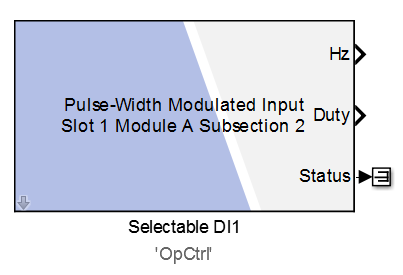
\includegraphics[width = 0.5\textwidth]{figures/PWM_in}
     \caption{PWM type digital input block diagram}
     \label{fig:pwm_in}
\end{figure}
\item \textbf{Event detection} \\
Event detection is capable of detect any digital event, including rising edge and failing edge which means we can use this feature to generate recover the input \gls{PWM}. In order to be able to convert event into \gls{PWM} signals, \Vref{fig:edge_detect} illustrates a nice way to archive the goal. The module can also generate time stamps when events occur. 
\begin{figure}[h]
     \centering
     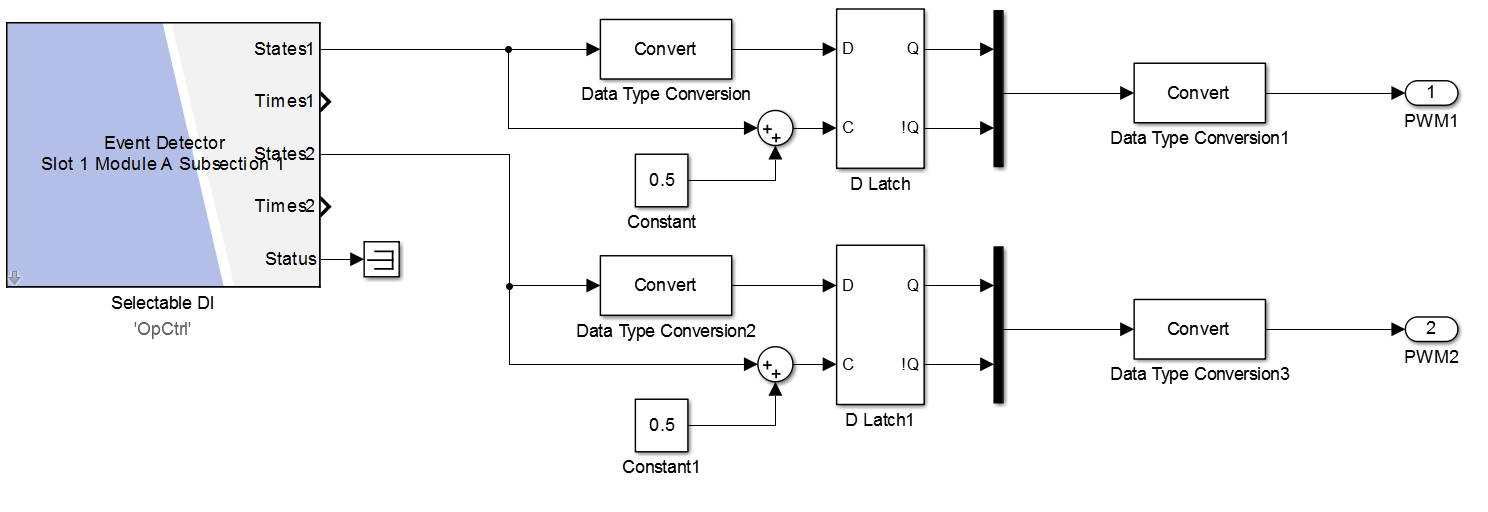
\includegraphics[width = 0.9\textwidth]{figures/event_detect}
     \caption{Edge dectection input block diagram}
     \label{fig:edge_detect}
\end{figure}
\end{enumerate}

In this project, the third approach (Event detection) is used and become a pitfall. The problem is that in this case the minimum time step of \gls{CPU} environment is set to $2e^{-5}$ s which is the minimum time step tried without getting overruns in the simulator, which lead to a maximum sampling frequency of digital input at 50 kHz. In this case, if a 25 kHz external \gls{PWM} is fed into the system, the duty cycle resolution is merely $\frac{50e^3}{25e^3}=2$, which is far more from sufficient. It was not until the closing stage of this project before this issue was found, which made it difficult to fix the issue due to limited time. 

One possible workaround for the problem encountered above is to feed external \gls{PWM} into \gls{FPGA} environment directly in stead of \gls{CPU} environment. \Vref{fig:fpga_digital} illustrates the available sources to control switching elements simulated using \gls{FPGA}. Although achievable minimum time step depends on model configuration, \ehs~can achieve average 250 ns of step size. Assuming minimum duty cycle variance is 1\% and it is possible to calculate the maximum external \gls{PWM} frequency is allowed. In this case, the frequency is $\frac{1}{250 \times 10 \times 10^{-9}}=400\ kHz$ which can be suitable for a wider range of simulation applications. Unfortunately, at the end of this project, this method has not been verified working yet. 
\begin{figure}[h]
     \centering
     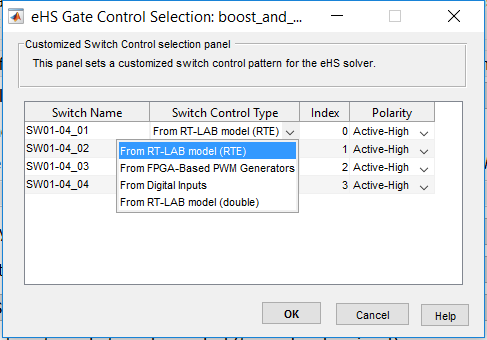
\includegraphics[width = 0.6\textwidth]{figures/fpga_digital}
     \caption{eHS gate source configurations}
     \label{fig:fpga_digital}
\end{figure}
\subsection{Test Setup}
\begin{figure}[h]
     \centering
     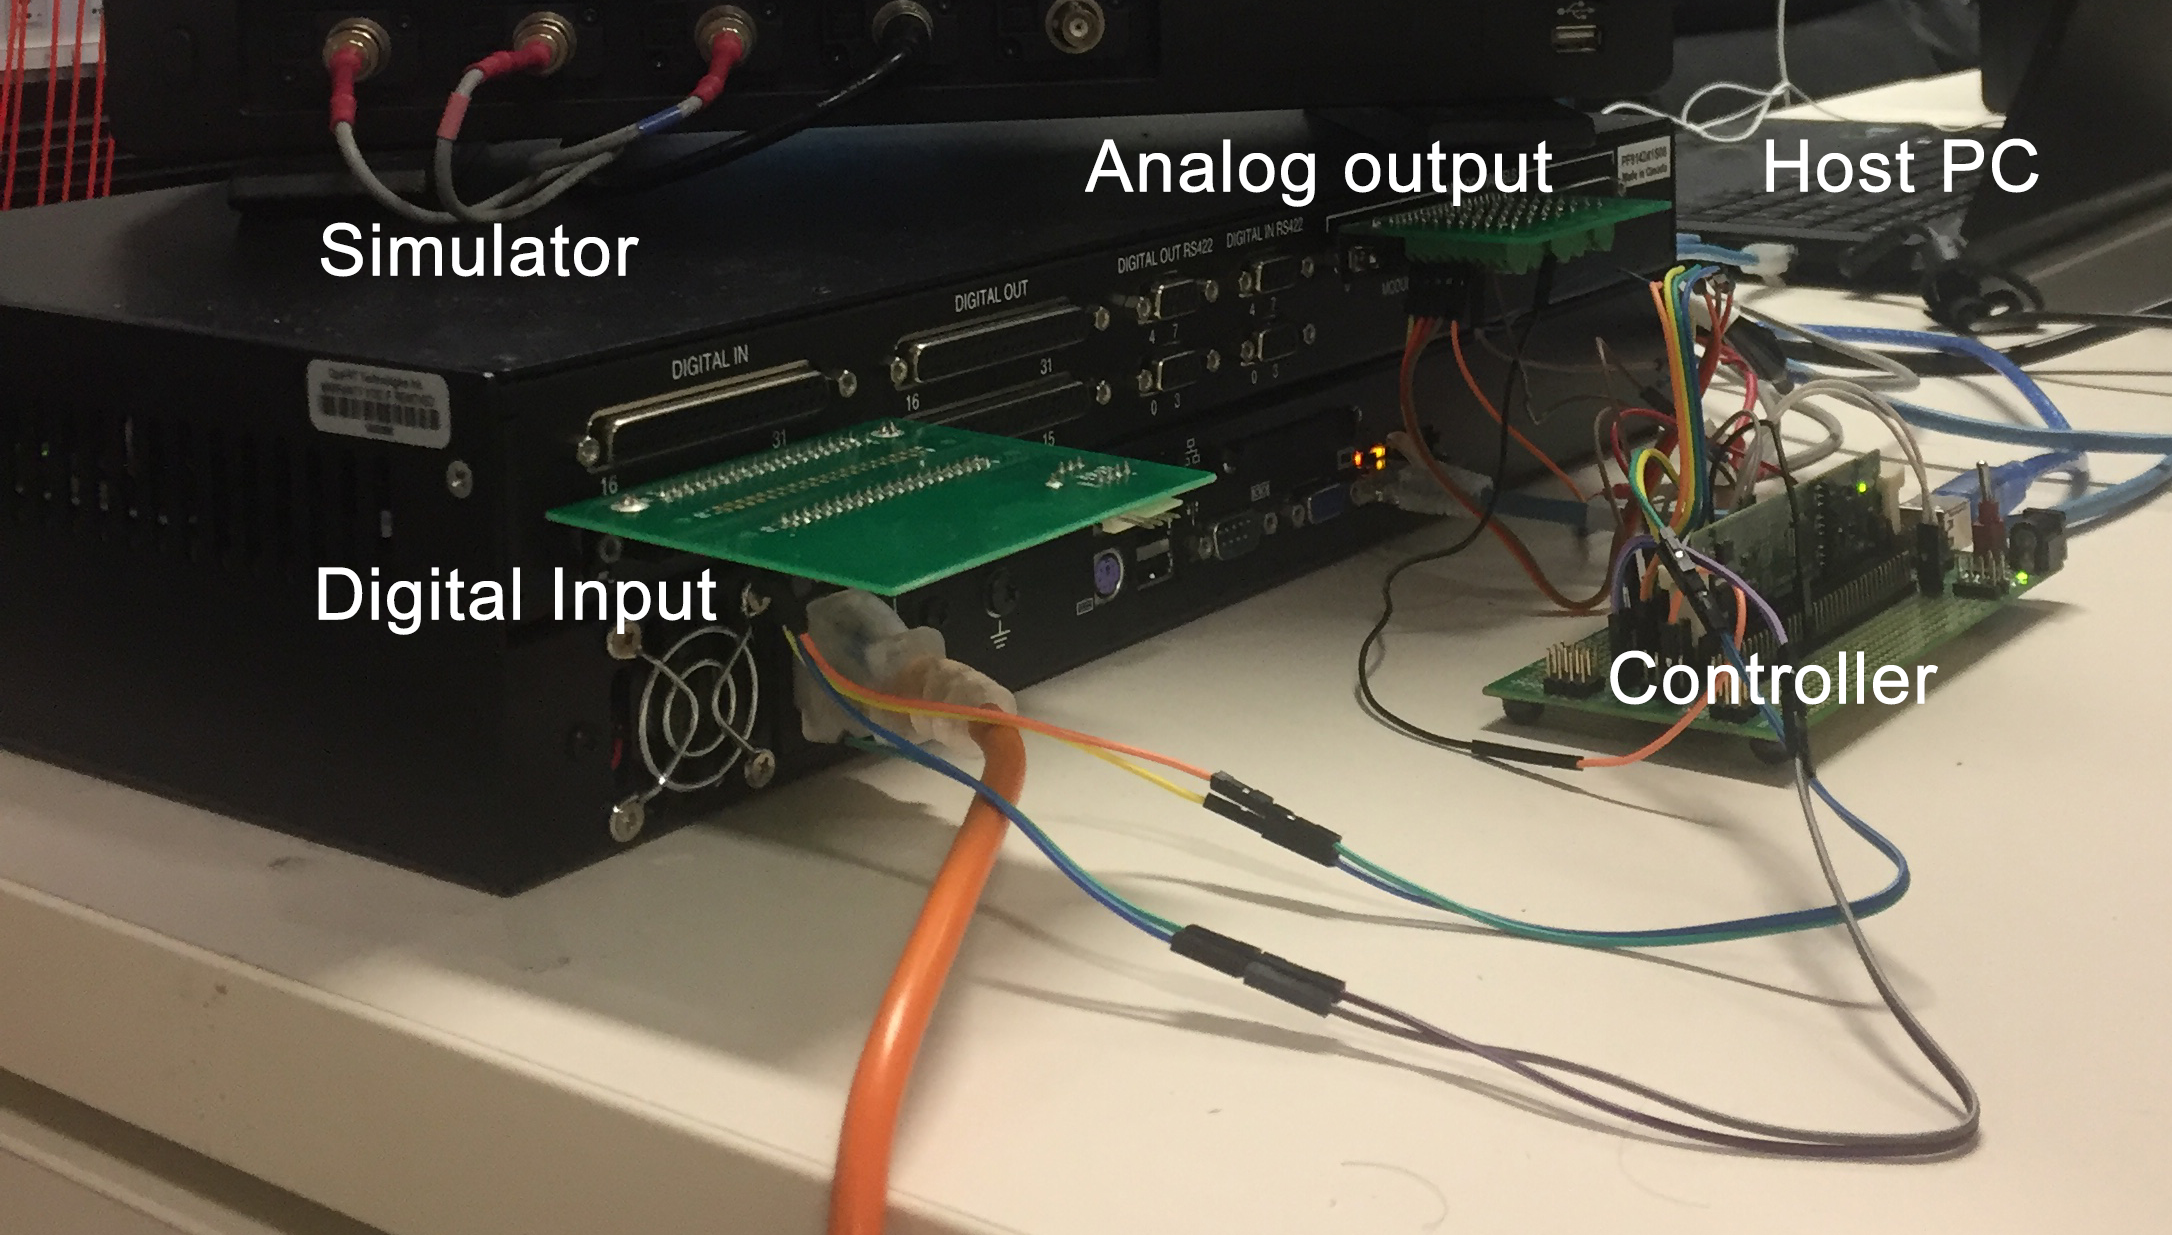
\includegraphics[width = 0.9\textwidth]{figures/setup}
     \caption{Simulation setup}
     \label{fig:setup}
\end{figure}
\Vref{fig:setup} illustrates the whole test setup for \gls{PIL} for this project. It clearly shows all the necessaries in order to perform \gls{PIL} simulation. Process required to run simulation are summarized here. 
\begin{enumerate}
\item \textbf{Setup wires} \\
Connect all wires required and it would be nice to use oscilloscope for debugging purpose. Double check wire connections to avoid making mistakes. 
\item \textbf{Upload model onto simulator} \\
Users have to upload loadable model onto simulator and make sure the simulator is ready to run simulation first. If the model is never ran before, it would be better if flag to force flush \gls{FPGA} firmware is turned on. Doing this can ensure we always have the up-to-date model being uploaded. However, programing \gls{FPGA} firmware takes more than five minutes which could lead to waste of precious time. 
\item \textbf{Program microcontroller} \\
\tms~may requires re-programming each time it gets powered up depending on RAM or FlASH version of binary file was previously programed. 
\item \textbf{Start running simulation} \\
Once the model is loaded and ready to run, users can start to run \gls{PIL} simulation. Waveforms can be accessed via host PC using auto-generated control console. It is more convenient to use oscilloscope to observe how model runs because communication bandwidth between host PC and simulator is so poor which makes it hard to use console for observation if more than five signals need to be watched. Once the model is running, simulator can be treated as virtual hardware and generated waveforms should be the same as expected. \\
\item \textbf{Stop simulation} \\
Once simulation is finished, users should always manually reset the simulator otherwise \rtlab~may crash and file results in the simulator may not be retrieved. 
\end{enumerate}
